\documentclass[11pt,a4paper]{article}
\usepackage[margin=22mm,headheight=14pt,footskip=12mm]{geometry}
\usepackage[T1]{fontenc}
\usepackage{lmodern,microtype,amsmath,booktabs,tabularx,array,tikz,enumitem,fancyhdr,url}
\usepackage[hidelinks]{hyperref}
\urlstyle{same}
\usetikzlibrary{arrows.meta,positioning,calc}
\setlength{\parindent}{0pt}
\setlength{\parskip}{5pt plus 1pt}
\setlist{nosep,leftmargin=1.5em,topsep=3pt,itemsep=3pt}
\usepackage[font=small,labelfont=bf]{caption}
\pagestyle{fancy}\fancyhf{}\renewcommand{\headrulewidth}{0pt}\fancyfoot[L]{\small OPEP research proposal \textbar\ Revision 0.3}
\fancyfoot[R]{\small\thepage}
\makeatletter
\renewcommand\section{\@startsection{section}{1}{\z@}{10pt plus 2pt minus 2pt}{4pt}{\normalfont\large\bfseries}}
\renewcommand\subsection{\@startsection{subsection}{2}{\z@}{7pt plus 2pt}{3pt}{\normalfont\normalsize\bfseries}}
\makeatother
\hypersetup{pdftitle={Development of a Modular Experimental Test Platform},pdfauthor={Abhijith Sivaprasadan},pdfsubject={Preliminary technical proposal for discussion}}
\begin{document}
\begin{center}
{\LARGE\bfseries Development of a Modular Experimental Test Platform\par}
\vspace{8pt}
{\large Abhijith Sivaprasadan\par}
Independent engineering project, Open Energy Methods\\
19 November 2026 \quad | \quad Preliminary technical proposal
\end{center}
\vspace{3pt}
\noindent\textbf{Abstract.} This proposal describes a personal engineering project to develop a small experimental platform for investigating the thermal behaviour of electronic components and assemblies. The initial work will concentrate on electrical and temperature measurements, heat transfer, precision manufacturing of fixtures, and comparison of measurements with analytical and numerical predictions. The platform is intended to be reconfigurable so that other investigations can be considered later, subject to resources and permissions. Particular attention will be given to measurement uncertainty, repeatability, boundary conditions and model validation. The project is undertaken in the author's spare time, without a fixed completion deadline. Designs, methods, software and data are intended for free public access where release is permitted. No experimental results are reported.

\section{Background and initial objectives}
Thermal predictions for electronic assemblies depend on the heat input, material properties, thermal contact between components, cooling conditions and the measurement locations. A nominal heat sink rating or a numerical temperature field is not sufficient to establish the actual performance of an assembly. A compact test fixture provides an opportunity to investigate these effects under documented conditions, while developing practical skills in machining, circuit assembly and instrumentation.

The initial question is whether a small, resource-constrained test arrangement can provide sufficiently repeatable electrical and thermal measurements to evaluate models of component heating and cooling. The first investigations would be limited to the following:
\begin{enumerate}
\item Characterize the electrical input and temperature measurement chain, including sensor attachment, response time and acquisition uncertainty.
\item Design, manufacture and inspect a fixture with repeatable mounting interfaces; assess how reassembly and manufacturing variation affect measured thermal behaviour.
\item Measure steady and transient thermal response at documented heat inputs and cooling conditions, and evaluate independently verified thermal models against measurements not used to fit model parameters.
\end{enumerate}
The existing Electronics Bench Testing (EBT) repository \cite{ebt} contains preliminary electrothermal designs and synthetic feasibility studies. It provides a starting point rather than validated hardware or measured data. A focused literature review will accompany the retained investigations before any claim of scientific novelty is made.

The Open Physical Engineering Programme (OPEP) is an independent hobby project. Practical work is intended for the KTH EECS Student Workshop, subject to local rules and permissions; this does not imply institutional sponsorship or approval of the proposed experiments.

\newpage
\section{Proposed apparatus and initial investigations}
The initial apparatus would use a replaceable heater assembly, heat sink, fixture and removable instrumentation on a compact base. A known resistive heat source is preferred for early measurements rather than beginning with an actively switched semiconductor. The arrangement should be dismantlable for storage in one box, excluding borrowed laboratory instruments. The base geometry and material will be chosen after inspection of the actual components and workshop stock; the earlier planning dimensions are not released manufacturing specifications.

\begin{center}
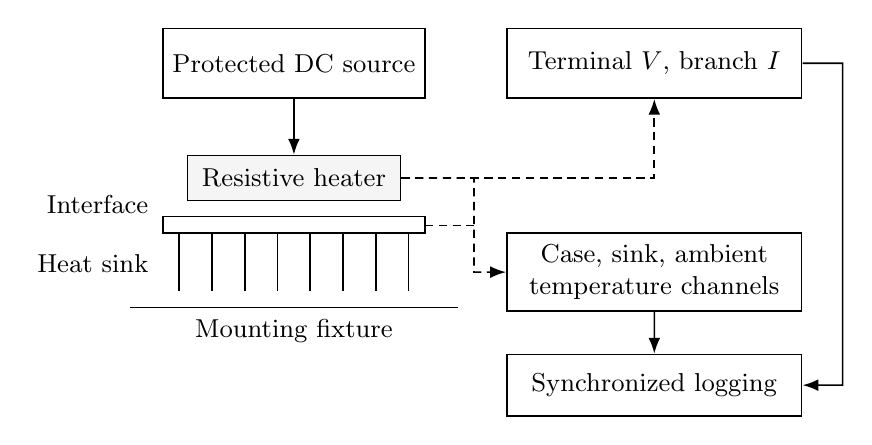
\begin{tikzpicture}[font=\small,>=Latex,line width=.6pt,scale=1.04,transform shape]
\node[draw,minimum width=3cm,minimum height=.85cm,align=center] (source) at (0,2.5) {Protected DC source};
\node[draw,minimum width=3.6cm,minimum height=.85cm,align=center] (meter) at (4.4,2.5) {Terminal $V$, branch $I$};
\node[draw,fill=gray!8,minimum width=2.6cm,minimum height=.55cm] (heater) at (0,1.1) {Resistive heater};
\draw[->] (source)--(heater);
\draw[densely dashed,->] (heater.east)-|(meter.south);
\draw (-1.6,.63) rectangle (1.6,.43);
\foreach \x in {-1.4,-1,-.6,-.2,.2,.6,1,1.4}{\draw (\x,.43)--(\x,-.28);}
\draw (-2,-.48)--(2,-.48);
\node[anchor=north] at (0,-.5) {Mounting fixture};
\node[anchor=east] at (-1.65,.05) {Heat sink};
\node[anchor=east] at (-1.65,.78) {Interface};
\node[draw,minimum width=3.6cm,minimum height=.95cm,align=center] (temp) at (4.4,-.05) {Case, sink, ambient\\temperature channels};
\draw[densely dashed,->] (heater.east)--(2.2,1.1)|-(temp.west);
\draw[densely dashed] (1.6,.52)--(2.2,.52);
\node[draw,align=center,minimum width=3.6cm,minimum height=.75cm] (daq) at (4.4,-1.43) {Synchronized logging};
\draw[->] (temp)--(daq);
\draw[->] (meter.east)--(6.7,2.5)|-(daq.east);
\end{tikzpicture}
\captionof{figure}{Conceptual measurement arrangement; not a wiring diagram or released hardware design. Cooling, protective devices, sensor positions and measurement ranges depend on the approved setup.}
\end{center}

\subsection{Manufacturing and assembly}
The first practical task is to inspect actual components and produce an appropriate fixture, with a specified datum, contact geometry and fastening arrangement. Dimensional inspection, material identification, tolerances, surface condition and assembly repeatability will be documented. Manual machining, CNC, printed supports or a milled PCB may be used where justified, following local training requirements. The objective is to assess the quality of the prototype and its assembly, not to certify an industrial production process from a small sample.

\subsection{Electrical and thermal measurements}
After confirmation of a permitted powered setup, the proposed measurements are heater-terminal voltage and branch current, heater-case and heat-sink temperatures, ambient temperature and time. The electrical input is $P_{\mathrm{el}}=VI$ for steady DC operation; transient input should be determined from time-aligned voltage and current. An apparent steady thermal resistance may be reported as $R_{\mathrm{app}}=(T_{\mathrm{case}}-T_{\mathrm{amb}})/P_{\mathrm{el}}$, with the configuration and measurement uncertainty stated. This is not an intrinsic convection coefficient or junction-to-ambient resistance. Lead losses, contact resistance, radiation and heat bypass must be considered. Natural cooling is the simplest candidate; forced cooling is optional if its boundary conditions can be characterized. No power or temperature limits are assigned by this proposal.

\newpage
\section{Measurement methodology and validation}
The measurement chain will be documented with instrument identity, operating range, calibration or verification evidence, sensor position, acquisition interval and synchronization. Pilot measurements should establish achievable signal-to-noise ratio, thermal response, drift and repeatability before a main test matrix is fixed. Independent assemblies or remounts will serve as experimental units where appropriate; repeated samples from a single transient are not independent replicates. Test order may be randomized or blocked, subject to safety and warm-up constraints \cite{nist}.

Measurement uncertainty will be evaluated following the principles of the GUM \cite{gum}. For a differentiable measurement model $y=f(x_1,\ldots,x_n)$, the first-order combined standard uncertainty is
\begin{equation}
 u_c^2(y)=\sum_{i=1}^n\sum_{j=1}^n
 \frac{\partial f}{\partial x_i}\frac{\partial f}{\partial x_j}\,\mathrm{cov}(x_i,x_j).
\end{equation}
Instrument specifications, calibration, sensor attachment, thermal lag, drift and correlated inputs will be considered as applicable. An experiment will be redesigned or its conclusions restricted if the measurement uncertainty is too large relative to the effect of interest.

The initial simulation work will use analytical heat balances and reduced-order thermal models, with finite-volume or finite-element heat transfer calculations where justified. Numerical verification will include conservation, limiting cases and spatial or temporal refinement, as applicable. Calibration and validation data should be separated by independent configurations or assemblies, with the predictive model fixed before assessing validation measurements. Prediction errors will be interpreted alongside experimental uncertainty and numerical error. Relevant ASME verification and validation guidance \cite{asme20} will inform the approach, without claiming formal conformity. A good fit to the calibration measurements alone is not independent validation.

\section{Availability, safety and practical feasibility}
The EECS Student Workshop lists metalworking, PCB milling, additive manufacturing and electrical bench equipment \cite{kthwork,kthmech,kthbio}. The presence of an equipment class does not establish its availability, calibration or suitability. Temperature instrumentation, synchronized acquisition, suitable dimensional references and independent cooling measurements still require confirmation. The first visit for the project will establish the actual instrument inventory and permissible work before committing to a fixture or purchasing components.

The project has no fixed schedule or deadline. Each investigation is subject to equipment, materials, funding, technical expertise, continued access and achievable measurement quality. Methods may be adapted, deferred or abandoned when essential resources cannot realistically be obtained; the reasons will be documented. A simpler experiment is preferable to a more elaborate arrangement with inadequate measurements.

All fabrication and tests require appropriate permissions and review. The workshop's rules require supervision for machining and prohibit working alone or on live circuits \cite{kthmech,kthsafe}. Powered work requires explicit permission for the proposed protected arrangement, or a separately authorized site. If that is unavailable, the powered investigation will be omitted or deferred. High-voltage, combustion, pressure-vessel, destructive and exposed high-speed rotating experiments are outside the present scope.

\newpage
\section{Possible future extensions}
The wider programme may be developed if the initial platform proves useful and suitable resources become available. These are possible independent investigations, not current deliverables or a fixed development sequence.
\begin{itemize}
\item Structural mechanics: force--deflection tests, joint compliance, strain measurement and comparison with finite element analysis.
\item Fluid mechanics and turbomachinery: guarded fan performance, duct pressure loss and CFD; gas-turbine-related thermodynamic modelling, performance analysis and suitable low-energy validation studies. Actual gas turbine or combustion testing is not proposed.
\item Control and diagnostics: system identification, feedback control, vibration, acoustics and condition monitoring, with suitable dynamic instrumentation.
\item Environmental and reliability studies, extended manufacturing and production investigations, and integration of validated models into a digital twin.
\end{itemize}
Each extension would require its own feasibility assessment, literature review, instrumentation and safety review. The initial thermal work does not depend on any of these extensions.

\section{Open work and technical feedback}
The intention is to make original engineering designs, calculations, methods, code, raw datasets with metadata and reports freely accessible under appropriate licences, subject to safety, ownership and facility permissions. Restrictions, failed tests and limitations will be documented. The private workshop manuals are not included in the public release.

Suggestions on practical thermal testing, sensor selection, fixture manufacturing, industrial measurement practices, comparable literature and methodological shortcomings are welcome. Potential contributors may propose work via the repository issue tracker and agree its scope with the maintainer before submitting changes for review. The proposal may be revised in response to feedback and practical feasibility. The repository is \url{https://github.com/Open-Energy-Methods/OPEP}.

\smallskip
\textbf{Declaration of AI assistance.} Generative AI was used to assist with preliminary planning, literature discovery, technical drafting and document preparation. The proposed methods, calculations and references remain subject to technical review and independent verification. Responsibility for engineering decisions and experimental work rests with the author.

\begingroup\small\setlength{\parskip}{1pt}
\begin{thebibliography}{99}\setlength{\itemsep}{2pt}\setlength{\parsep}{0pt}
\bibitem{ebt} Open Energy Methods, \emph{Electronics Bench Testing}, existing independent design and synthetic feasibility repository. \href{https://github.com/Open-Energy-Methods/electronics-bench-testing}{GitHub repository}.
\bibitem{nist} NIST/SEMATECH, \emph{e-Handbook of Statistical Methods}, Sec. 5.3, Choosing an experimental design. \href{https://www.itl.nist.gov/div898/handbook/pri/section3/pri3.htm}{Online handbook}.
\bibitem{gum} JCGM 100:2008, \emph{Evaluation of measurement data---Guide to the expression of uncertainty in measurement}. \href{https://doi.org/10.59161/JCGM100-2008E}{doi:10.59161/JCGM100-2008E}.
\bibitem{asme20} ASME V\&V 20, \emph{Standard for Verification and Validation in Computational Fluid Dynamics and Heat Transfer}. \href{https://www.asme.org/codes-standards/find-codes-standards/standard-for-verification-and-validation-in-computational-fluid-dynamics-and-heat-transfer}{ASME standard listing}.
\bibitem{kthwork} KTH, \emph{Explore KTH's makerspaces}. \href{https://www.kth.se/en/student/kontakt/campus/makerspaces/explore/explore-1.1455863}{Student Workshop listing}. Accessed 19 Nov. 2026.
\bibitem{kthmech} KTH, \emph{Student Workshop: Mechanical manufacturing}. \href{https://www.kth.se/emp/student-workshop/verkstan/mekanik-1.686913}{Equipment and supervision}. Accessed 19 Nov. 2026.
\bibitem{kthbio} KTH, \emph{Student Workshop: Electronics}. \href{https://www.kth.se/emp/student-workshop/verkstan/elektronik-1.686912}{Electronics equipment}. Accessed 19 Nov. 2026.
\bibitem{kthsafe} KTH, \emph{Student Workshop: Order and Safety Rules}. \href{https://www.kth.se/emp/student-workshop/regler-och-sakerhet}{Safety rules}. Accessed 19 Nov. 2026.
\end{thebibliography}\endgroup
\end{document}
